% -*- mode: fundamental -*-

% Slides accompanying "Learn RISC-V CPU Implementation and BSV" book
% Copyright (c) 2024 Rishiyur S. Nikhil, All Rights Reserved

% -*- mode: fundamental -*-

% Slides accompanying "Learn RISC-V CPU Implementation and BSV" book
% Copyright (c) 2024 Rishiyur S. Nikhil, All Rights Reserved

% This is a preamble shared by all the slide decks

\documentclass[10pt, aspectratio=169]{beamer}

% \documentclass[17pt]{beamer}

% Avail. font sizes: 8pt, 9pt, 10pt, 11pt, 12pt, 14pt, 17pt, 20pt.
% Default font size is 11pt (= 22pt in full screen mode).

\usepackage{verbatim}
\usepackage{fancyvrb}
\usepackage{listings}

% ================================================================
% Themes

\usetheme{Madrid}          % Line at bottom: Author (affiliation), OptTitle, Conf, page 

% \usetheme{Copenhagen}    % Same as Madrid except bottom line: Author, OptTitle

% \usetheme{Berkeley}    % Takes up 1-inch border on left and top

% ----------------
% colorthemes
% (default), beaver, beetle, seahorse, wolverine

\usecolortheme{seahorse}

% ================================================================
% Customization: show table of contents before each section
% Use \AtBeginSubsection    to show before each subsection

% \AtBeginSection[]
% {
%   \begin{frame}
%     \frametitle{Table of Contents}
%     \tableofcontents[currentsection]
%   \end{frame}
% }

% ================================================================

% ----------------
% The bsc compiler and BSV language
\newcommand{\bsc}{\emph{bsc}}
\newcommand{\BSV}{\bf{BSV}}
% ----------------
% ITALICISE WORDS
\newcommand{\ie}{\emph{i.e.,}}
\newcommand{\eg}{\emph{e.g.,}}
\newcommand{\Eg}{\emph{E.g.,}}
\newcommand{\etc}{\emph{etc.}}
\newcommand{\via}{\emph{via}}
\newcommand{\vs}{\emph{vs.}}

% ----------------
% EMPTY BOXES OF VARIOUS WIDTHS, FOR INDENTATION

\newcommand{\hm}{\hspace*{1em}}
\newcommand{\hmm}{\hspace*{2em}}
\newcommand{\hmmm}{\hspace*{3em}}
\newcommand{\hmmmm}{\hspace*{4em}}

% ----------------
% Convenient widths

\newlength{\hlessmm}
\setlength{\hlessmm}{\textwidth}
\addtolength{\hlessmm}{-2em}

\newlength{\hlessmmm}
\setlength{\hlessmmm}{\textwidth}
\addtolength{\hlessmmm}{-3em}

\newlength{\hlessmmmm}
\setlength{\hlessmmmm}{\textwidth}
\addtolength{\hlessmmmm}{-4em}

% ================================================================
% Title page

\title[Learn CPU design \& BSV]{Learn RISC-V CPU Implementation and BSV}

\subtitle{(BSV: a High-Level Hardware Design Language)}

\author[{\copyright} R.S.Nikhil]{Rishiyur S.~Nikhil}
% \institute{Bluespec, Inc.}

% Date is set differently in each slide deck

% \logo{
\includegraphics[height=0.6cm]{../Figures/Bluespec_Logo_2022-10}}

% End of preamble
% ****************************************************************


\date{L6: RISC-V: Core functions for ISA execution}

% ****************************************************************

\begin{document}

% ================================================================

\begin{frame}
 \titlepage

 \begin{center}
  
\includegraphics[height=1cm]{Bluespec_Logo_2022-10}
 \end{center}

\end{frame}

% ================================================================

% -*- mode: fundamental -*-

% ================================================================

\begin{frame}[fragile]
\frametitle{Reminders}

\footnotesize

Please git clone: \url{https://github.com/rsnikhil/Learn_Bluespec_and_RISCV_Design} \\
(git pull for latest version).  Repsitory structure:

\vspace{1ex}

\begin{minipage}{0.5\textwidth}\scriptsize
\begin{Verbatim}[frame=single, numbers=left]
    ./Book_BLang_RISCV.pdf
      Slides/
          Slides_01_Intro.pdf
          Slides_02_ISA.pdf
          ...
      Exercises/
          Ex-03-A-Hello-World/
          Ex-03-B-Top-and-DUT/
          ...
      Code/
          src_Top/
          src_Drum/
          src_Fife/
          src_Common/
          ...
      Doc/Installing_bsc_Verilator_etc.{adoc,html}
\end{Verbatim}
\end{minipage}
\hm
\begin{minipage}{0.45\textwidth}
\begin{itemize}

 \item Slides and Exercise are numbered in sync with book Chapter numbers.

 \item For Exercises, please see Appendix E of the book.  Some (not
       all) exercises have associated code in the {\tt Exercises/}
       directory.

\end{itemize}
\end{minipage}

\vspace{2ex}

To compile and run the code for exercises, Drum and Fife, please make sure you have installed:

\begin{itemize}

 \item \emph{bsc} compiler (see \url{https://github.com/B-Lang-org/bsc})

 \item Verilator compiler (see \url{https://www.verilator.org/})
\end{itemize}

\footnotesize

\end{frame}

% ================================================================

\begin{frame}
\frametitle{Chapter Roadmap}

\footnotesize

\begin{center}
\frame{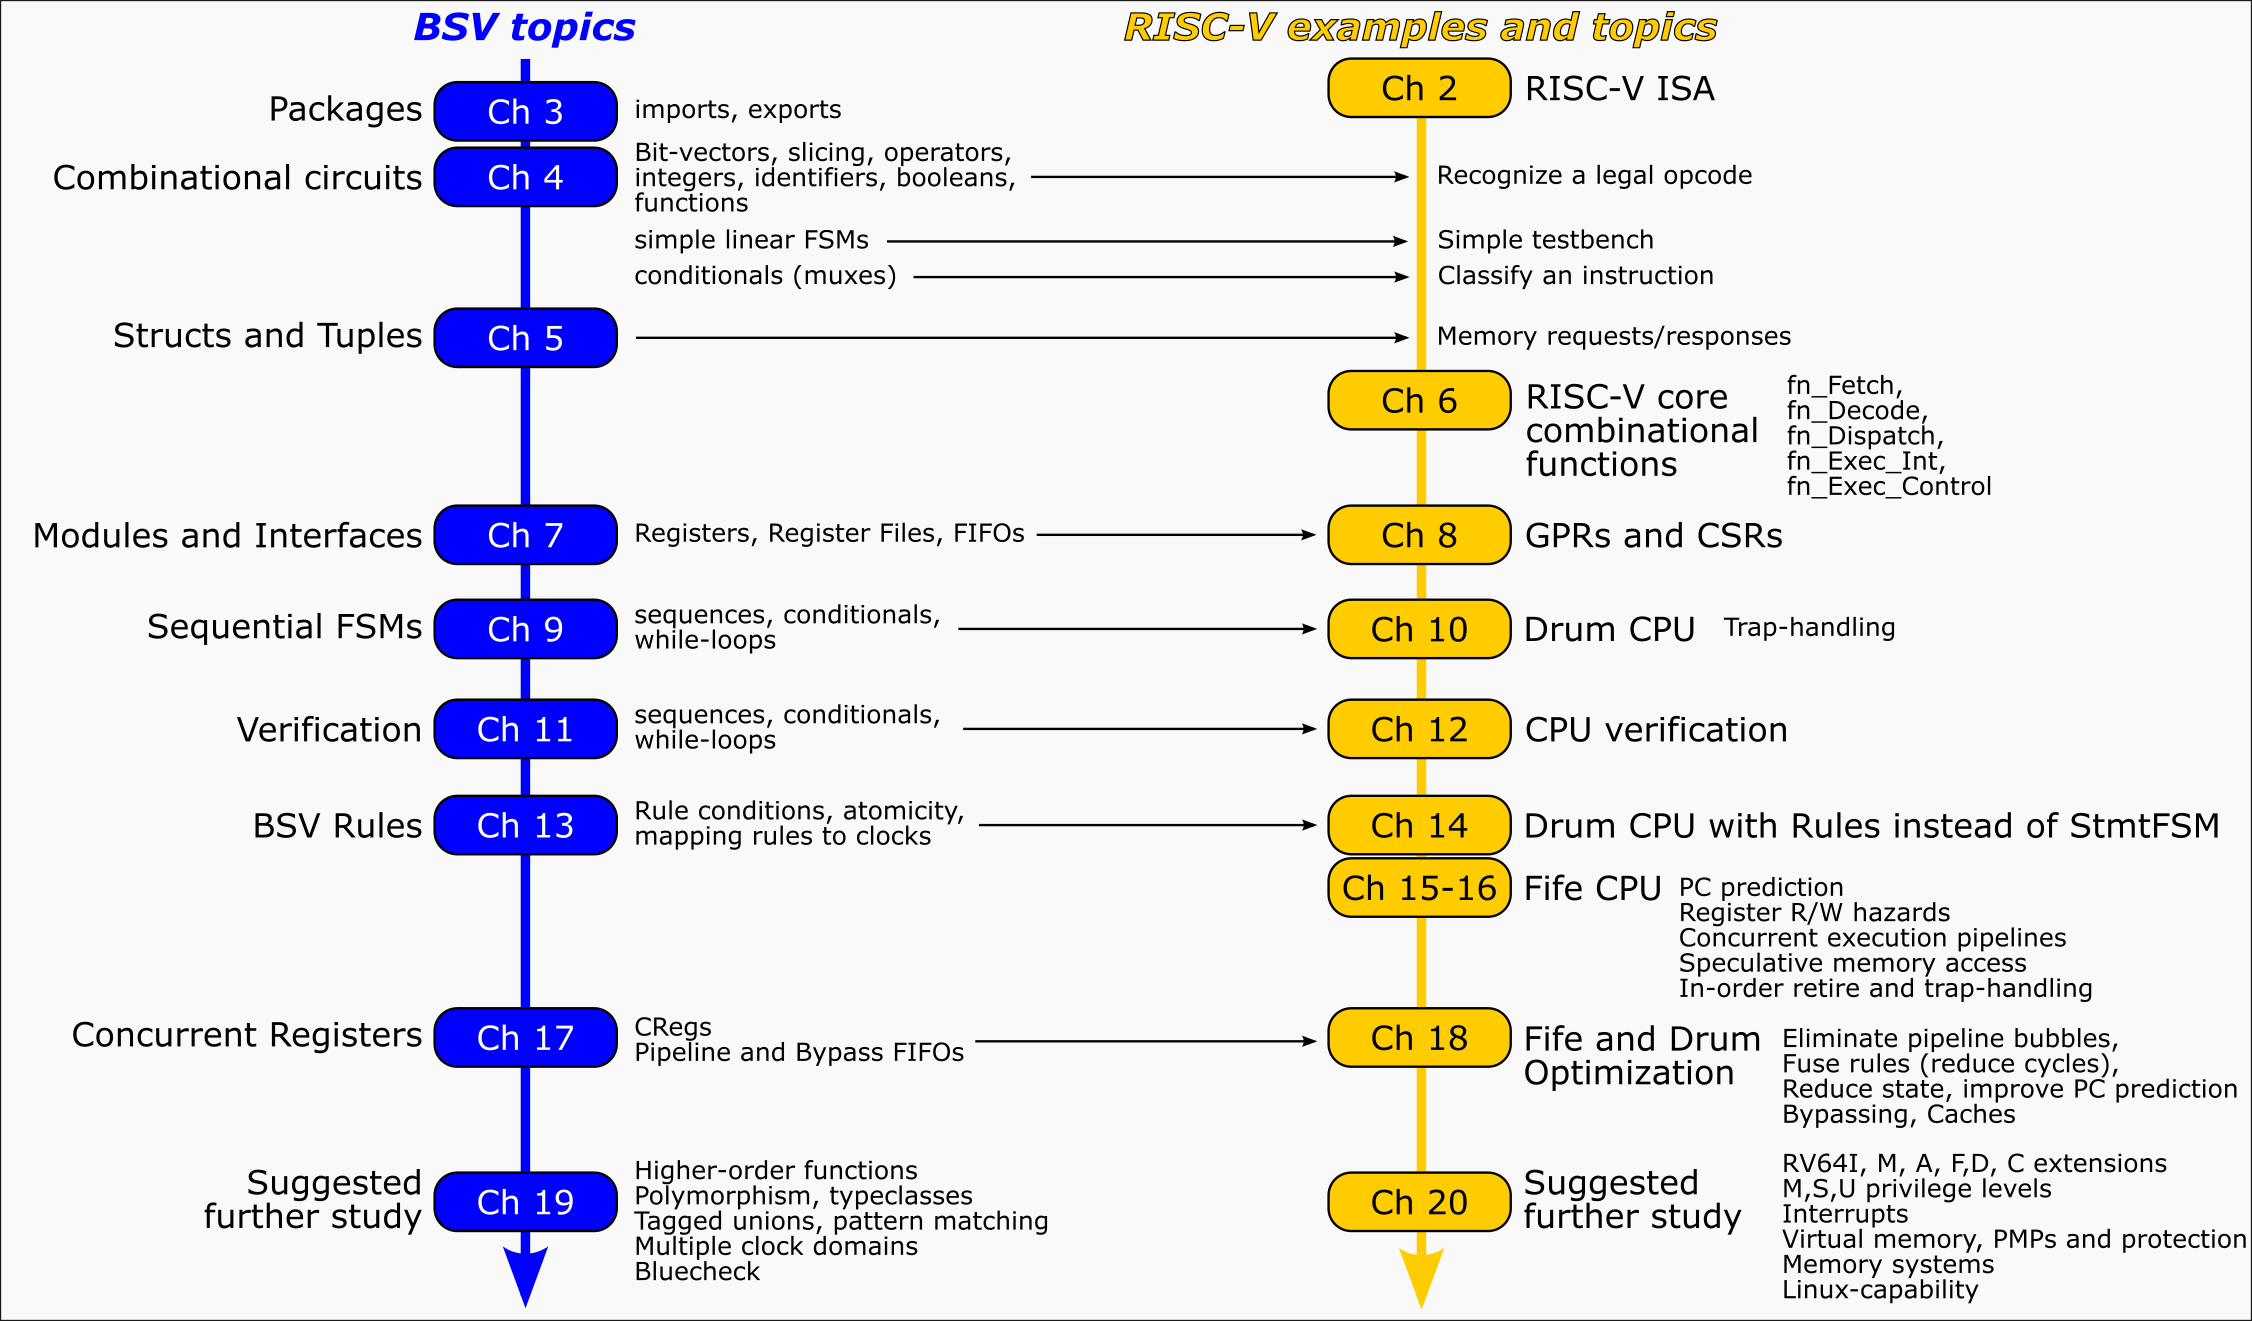
\includegraphics[height=0.825\textheight]{Fig_Chapter_Roadmap}}
\end{center}

\end{frame}

% ================================================================


% ================================================================

\begin{frame}
\frametitle{Flow of information between stages in Drum and Fife}

\footnotesize

\begin{center}
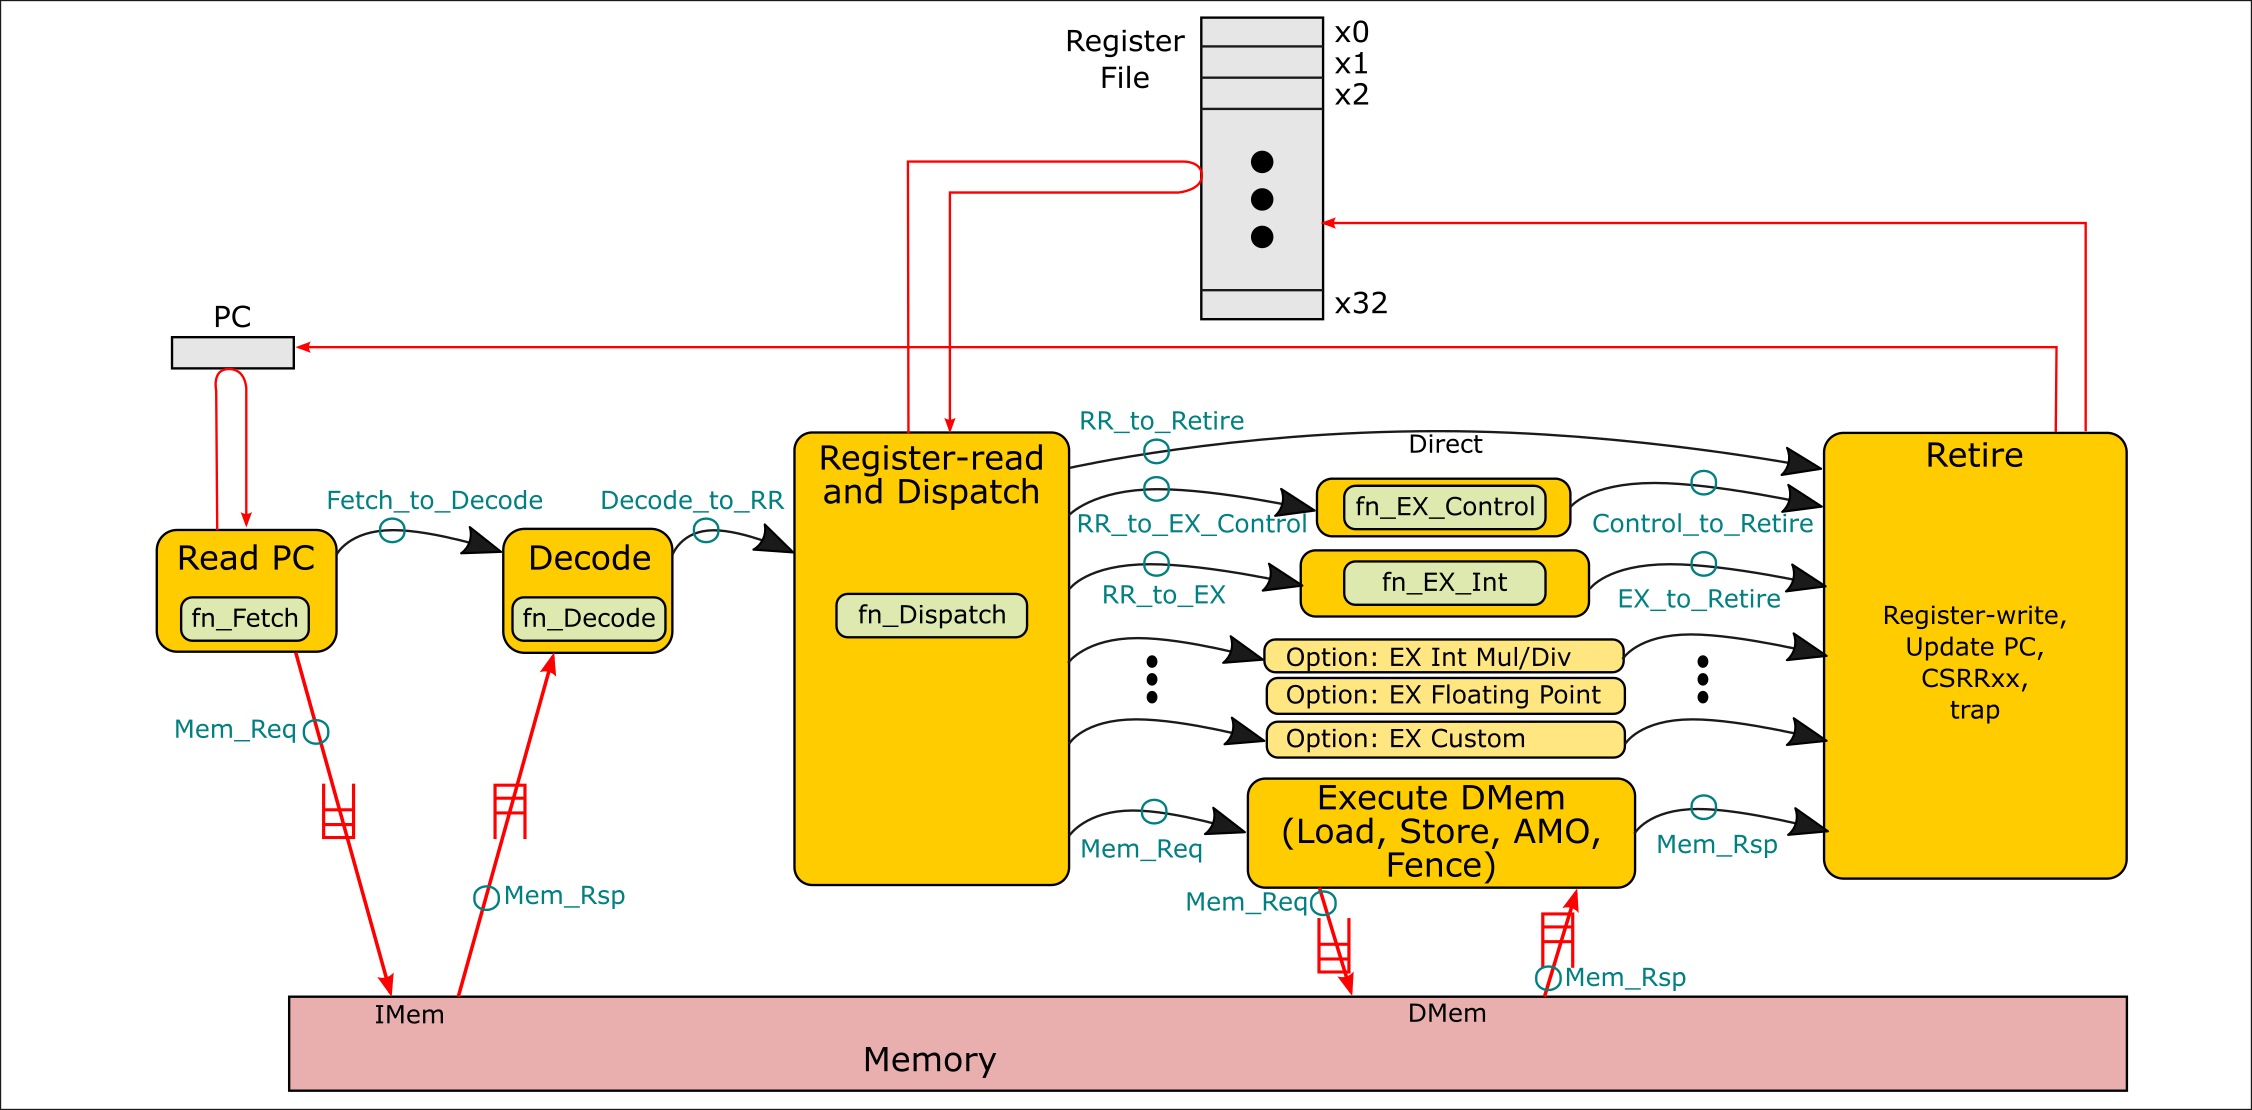
\includegraphics[height=0.6\textheight]{Fig_Instr_Exec_w_structs}
\end{center}

\vspace*{2ex}

The green annotations indicate the type of information flowing on each arrow.

Each of these is a ``{\tt struct}'' type (also known as a ``record''):
a heterogeneous grouping of \emph{fields} of various types.

\end{frame}

% ================================================================

\begin{frame}
\frametitle{Table of Contents}

\tableofcontents

\end{frame}

% ****************************************************************

\section{Fetch}

\begin{frame}

\begin{center}
  {\LARGE\tt fn\_Fetch}

  \vspace{5ex}

  Excerpts shown in next few slides.

  Please also view the actual code in:
  {\tt Code/src\_Common/Fn\_Fetch.bsv}

\end{center}

\end{frame}

% ================================================================

\begin{frame}[fragile]
\frametitle{Inputs and outputs of {\tt fn\_Fetch}}

\footnotesize

Direct output from {\tt fn\_Fetch} to Decode:

\vspace{1ex}

\SHOWCODE{../Code_Extracts/Fetch_to_Decode.tex}

\vspace{5ex}

Overall output of {\tt fn\_Fetch}

\vspace{1ex}

\SHOWCODE{../Code_Extracts/Result_F.tex}

\end{frame}

% ================================================================

\begin{frame}
\frametitle{{\tt fn\_Fetch}}

\footnotesize

\SHOWCODE{../Code_Extracts/Fn_Fetch.tex}

\end{frame}

% ================================================================

\begin{frame}[fragile]
\frametitle{{\tt fn\_Fetch} is actually a pure function}

\footnotesize

{\tt fn\_Fetch} is actually a pure (side effect-free) function and
could have been written without {\tt ActionValue\#()}:

\vspace{2ex}

\begin{minipage}{0.45\textwidth}
 \begin{Verbatim}[frame=single]
function ActionValue #(Result_F)
         fn_Fetch (Bit #(XLEN)  pc,
                   ...
                   Bit #(64)    inum);
   actionvalue
      Result_F y = ?;
      ...
      return y;
   endactionvalue
endfunction
 \end{Verbatim}
\end{minipage}
\hfill
$\Longrightarrow$
\hfill
\begin{minipage}{0.45\textwidth}
 \begin{Verbatim}[frame=single]
function Result_F
         fn_Fetch (Bit #(XLEN)  pc,
                   ...
                   Bit #(64)    inum);
      Result_F y = ?;
      ...
      return y;
endfunction
 \end{Verbatim}
\end{minipage}

\vspace{2ex}

We write it this way only to make it easy to add {\tt \$display()}
statements for debugging in case we need them (when {\tt
ActionValue\#()} would be necessary).

\end{frame}

% ================================================================

\begin{frame}
\frametitle{\EmojiExercise \hmm Exercise break}

Please see Appendix E, Section Ex-06-A-Fetch.

\end{frame}

% ****************************************************************

\section{Decode}

% ================================================================

\begin{frame}

\begin{center}
  {\LARGE\tt fn\_Decode}

  \vspace{5ex}

  Excerpts shown in next few slides.

  Please also view the actual code in:
  {\tt Code/src\_Common/Fn\_Decode.bsv}

\end{center}

\end{frame}

% ================================================================

\begin{frame}[fragile]
\frametitle{Output of {\tt fn\_Decode}}

\footnotesize

\SHOWCODE{../Code_Extracts/Decode_to_RR.tex}

\end{frame}

% ================================================================

\begin{frame}
\frametitle{Fields of struct {\tt Decode\_to\_RR}}

\footnotesize

\begin{itemize}

 \item The current PC: will be needed by BRANCH, JAL, AUIPC to compute
       a target address relative to the current PC.

 \PAUSE{\vspace{1ex}}

 \item Was there an exception (Fetch memory error, or instruction is not legal)?
       If so, what was the cause?

 \PAUSE{\vspace{1ex}}

 \item If no exception, what is the fall-through PC (needed for
       next-PC update for most instructions, and for saved-PC
       (``return address'') for JAL/JALR).

 \PAUSE{\vspace{1ex}}

 \item What is the instruction?  What is its broad classification:
       Control (Branch or Jump)? Integer Arithmetic or Logic? Memory
       Access?  This will help in choosing the execute stage pipeline.

 \PAUSE{\vspace{1ex}}

 \item Does it have zero, one or two input registers (``rs1'' and
       ``rs2'')?  If so, which ones?  This will help the Register-Read
       stage in reading registers and, for Fife, for managing ``hazards''.

 \PAUSE{\vspace{1ex}}

 \item Does it have zero or one output registers (``rd'')?  If so,
       which one?  This will help the final Register Write stage in
       writing back a value to a register.

 \PAUSE{\vspace{1ex}}

 \item Does it write memory?  In Fife, where we do speculative writes
       to memory, this will help the Retire stage commit (finalize)
       those writes.

 \PAUSE{\vspace{1ex}}

 \item What is the ``immediate'' value, if any (after untangling all
       different ways in which bits are permuted in different formats of
       instructions.

\end{itemize}

\end{frame}

% ================================================================

\begin{frame}[fragile]
\frametitle{Fields of struct {\tt Decode\_to\_RR}}

\footnotesize

Some {\tt Decode\_to\_RR} fields, such as \verb|has_rs1|, are used in
later stages, and could be computed there from \verb|instr|; so why
compute them here in Decode?

\vspace{4ex}

\begin{itemize}

 \item If something is needed in more than one stage, computing it
       once and carrying the value forward can save some hardware cost
       (gates).  It also incurs a hardware cost: we have to allocate
       state elements for the carried value in each inter-stage
       buffer/FIFO.

 \item Wherever something is computed, it adds to combinational delay
       for that stage (lowering achievable clock speed).

\end{itemize}

\vspace{4ex}

The decision between compute-and-carry {\vs} compute later is a
balancing act between these kinds of considerations.

\end{frame}

% ================================================================

\begin{frame}
\frametitle{{\tt fn\_Decode}}

\footnotesize

\begin{center}\large
 Please view the actual code in: \hm {\tt Code/src\_Common/Fn\_Decode.bsv}
\end{center}

\end{frame}

% ================================================================

\begin{frame}
\frametitle{\EmojiExercise \hmm Exercise break}

Please see Appendix E, Section Ex-06-B-Decode.

\end{frame}

% ****************************************************************

\section{Dispatch}

\begin{frame}

\begin{center}
  {\LARGE\tt fn\_Dispatch}

  \vspace{5ex}

  Excerpts shown in next few slides.

  Please also view the actual code in:
  {\tt Code/src\_Common/Fn\_Dispatch.bsv}

\end{center}

\end{frame}

% ================================================================

\begin{frame}[fragile]
\frametitle{Partial output of {\tt fn\_Dispatch}: direct to Retire}

\footnotesize

\SHOWCODE{../Code_Extracts/RR_to_Retire.tex}

\end{frame}

% ================================================================

\begin{frame}[fragile]
\frametitle{Partial output of {\tt fn\_Dispatch}: to Execute-Control}

\footnotesize

\SHOWCODE{../Code_Extracts/RR_to_EX_Control.tex}

\end{frame}

% ================================================================

\begin{frame}[fragile]
\frametitle{Partial output of {\tt fn\_Dispatch}: to Execute-Integer ALU}

\footnotesize

\SHOWCODE{../Code_Extracts/RR_to_EX.tex}

\end{frame}

% ================================================================

\begin{frame}[fragile]
\frametitle{Partial output of {\tt fn\_Dispatch}: to Execute-Integer ALU}

\footnotesize

\SHOWCODE{../Code_Extracts/RR_to_EX.tex}

\end{frame}

% ================================================================

\begin{frame}[fragile]
\frametitle{Full output of {\tt fn\_Dispatch}}

\footnotesize

\SHOWCODE{../Code_Extracts/Result_Dispatch.tex}

\end{frame}

% ================================================================

\begin{frame}
\frametitle{{\tt fn\_Dispatch}}

\footnotesize

\begin{center}\large
 Please view the actual code in: \hm {\tt Code/src\_Common/Fn\_Dispatch.bsv}
\end{center}

\end{frame}

% ================================================================

\begin{frame}
\frametitle{\EmojiExercise \hmm Exercise break}

Please see Appendix E, Section Ex-06-C-Dispatch.

\end{frame}

% ****************************************************************

\section{Execute Control}

\begin{frame}[fragile]

\begin{center}
  {\LARGE\tt fn\_Ex\_Control}

  \vspace{5ex}

  Excerpts shown in next few slides.

  Please also view the actual code in:
  {\tt Code/src\_Common/Fn\_Ex\_Control.bsv}

\end{center}

\end{frame}

% ================================================================

\begin{frame}[fragile]
\frametitle{Output of {\tt fn\_Ex\_Control}}

\footnotesize

\SHOWCODE{../Code_Extracts/EX_Control_to_Retire.tex}

\end{frame}

% ================================================================

\begin{frame}
\frametitle{{\tt fn\_Ex\_Control}}

\footnotesize

\begin{center}\large
 Please view the actual code in: \hm {\tt Code/src\_Common/Fn\_Ex\_Control.bsv}
\end{center}

\end{frame}

% ================================================================

\begin{frame}
\frametitle{\EmojiExercise \hmm Exercise break}

Please see Appendix E, Section Ex-06-D-Ex-Control.

\end{frame}

% ****************************************************************

\section{Execute Int}

\begin{frame}[fragile]

\begin{center}
  {\LARGE\tt fn\_Ex\_Int}

  \vspace{5ex}

  Excerpts shown in next few slides.

  Please also view the actual code in:
  {\tt Code/src\_Common/Fn\_Ex\_Int.bsv}

\end{center}

\end{frame}

% ================================================================

\begin{frame}[fragile]
\frametitle{Output of {\tt fn\_Ex\_Int}}

\footnotesize

\SHOWCODE{../Code_Extracts/EX_to_Retire.tex}

\end{frame}

% ================================================================

\begin{frame}
\frametitle{{\tt fn\_Ex\_Int}}

\footnotesize

\begin{center}\large
 Please view the actual code in: \hm {\tt Code/src\_Common/Fn\_Ex\_Int.bsv}
\end{center}

\end{frame}

% ================================================================

\begin{frame}
\frametitle{\EmojiExercise \hmm Exercise break}

Please see Appendix E, Section Ex-06-E-Ex-Int.

\end{frame}

% ****************************************************************

% -*- mode: fundamental -*-

% Slides accompanying "Learn RISC-V CPU Implementation and BSV" book
% Copyright (c) 2024 Rishiyur S. Nikhil, All Rights Reserved

% This is a postamble shared by all the slide decks

% ================================================================

\begin{frame}

\begin{center}
  {\LARGE End}
\end{center}

\end{frame}

% ================================================================


% ****************************************************************

\end{document}
